\tikzstyle{txt} = [text centered, inner sep=0pt]

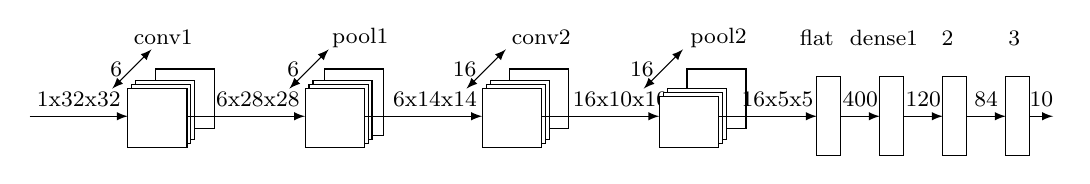
\begin{tikzpicture}[scale=1.0,
z={({0.3cm*cos(45)},{0.3cm*sin(45)})},
>=latex, 
font=\footnotesize,
]

% Big Input images



%CONV1
\draw[fill=white] (0.25+7*0.05,7*0.05) rectangle (1+7*0.05,.75+7*0.05);
\foreach \foreach \z in {2,...,0}  {%
 \draw[fill=white] (0.25+\z*0.05,.1+\z*0.05) rectangle (1+\z*0.05,.85+\z*0.05);
}
\draw (0.7,1.5)node[txt] (conv1){conv1};
\draw[->] (-1,0.5) -- node[above] {$1$x$32$x$32$} (0.25,0.5);
\draw[<->] (.25-0.2,.85+0*0.05) -- node[left] {$6$} (.25+0.3,.85+0.5);

%MAXPOOL1
\draw[fill=white] (2.5+5*0.05,5*0.05) rectangle (3.25+5*0.05,0.85+5*0.05);
\foreach \foreach \z in {2,...,0}  {%
 \draw[fill=white] (2.5+\z*0.05,0.1+\z*0.05) rectangle (3.25+\z*0.05,.85+\z*0.05);
}
\draw (3.2,1.5)node[txt] (conv1){pool1};
\draw[->] (1,0.5) -- node[above,pos=0.6] {$6$x$28$x$28$} (2.5,0.5);
\draw[<->] (2.5-0.2,0.85+0*0.05) -- node[left] {$6$} (2.5+0.3,0.85+0.5);

%CONV2
\draw[fill=white] (4.75+7*0.05,7*0.05) rectangle (5.5+7*0.05,0.75+7*0.05);
\draw (5.5,1.5)node[txt] (conv1){conv2};
\draw[->] (3.25,0.5) -- node[above,pos=0.6] {$6$x$14$x$14$} (4.75,0.5);
\foreach \foreach \z in {2,...,0}  {%
 \draw[fill=white] (4.75+\z*0.05,0.1+\z*0.05) rectangle (5.5+\z*0.05,0.85+\z*0.05);
}
\draw[<->] (4.75-0.2,0.85+0*0.05) -- node[left] {$16$} (4.75+0.3,0.85+0.5);

%MAXPOOL2
\draw[fill=white] (7+7*0.05,7*0.05) rectangle (7.75+7*0.05,0.75+7*0.05);
\draw[->] (5.5,0.5) -- node[above,pos=0.67] {$16$x$10$x$10$} (7,0.5);
\foreach \foreach \z in {2,...,0}  {%
 \draw[fill=white] (7+\z*0.05,0.1+\z*0.05) rectangle (7.75+\z*0.05,0.75+\z*0.05);
}
\draw (7.75,1.5)node[txt] (conv1){pool2};
\draw[<->] (7-0.2,0.85+0*0.05) -- node[left] {$16$} (7+0.3,0.85+0.5);
\draw[->] (7.75,0.5) -- node[above,pos=0.6] {$16$x$5$x$5$} (9,0.5);

\draw[fill=white] (9,0) rectangle (9.3,1);
\draw[->] (9.3,0.5) -- node[above] {$400$} (9.8,0.5);
\draw (9,1.5)node[txt] (conv1){flat};

%dense1
\draw[fill=white] (9.8,0) rectangle (10.1,1);
%dense2
\draw[fill=white] (10.6,0) rectangle (10.9,1);
%dense3
\draw[fill=white] (11.4,0) rectangle (11.7,1);
\draw[->] (10.1,0.5) --node[above] {$120$}(10.6,0.5);
\draw[->] (10.9,0.5) --node[above] {$84$} (11.4,0.5);
\draw (10.5,1.5)node[txt] (conv1){dense1 \hspace{.1cm} 2 \hspace{.5cm} 3};



\draw[->] (11.7,0.5) -- node[above] {$10$} (12,0.5);




\end{tikzpicture}
